%!TEX root = ../MasterThesis.tex

\section{Data flow for credit card transactions}
\label{sec:stakeholder_data_flow}

As the previous chapter shows, there are a many stakeholders involved in providing \gls{IT} hardware, software and services to keep the Web shops on the Internet up and running. Only a small fraction of those will have to deal with the handling of credit card payments and order fulfillment though. These are the relevant stakeholders to look at in the case of an \gls{E-commerce} fraud incident. The actual flow of information between them is displayed in  Figure~\ref{fig:images_e_commerce_stakeholder}. \@

\begin{figure}[H]
	\centering
		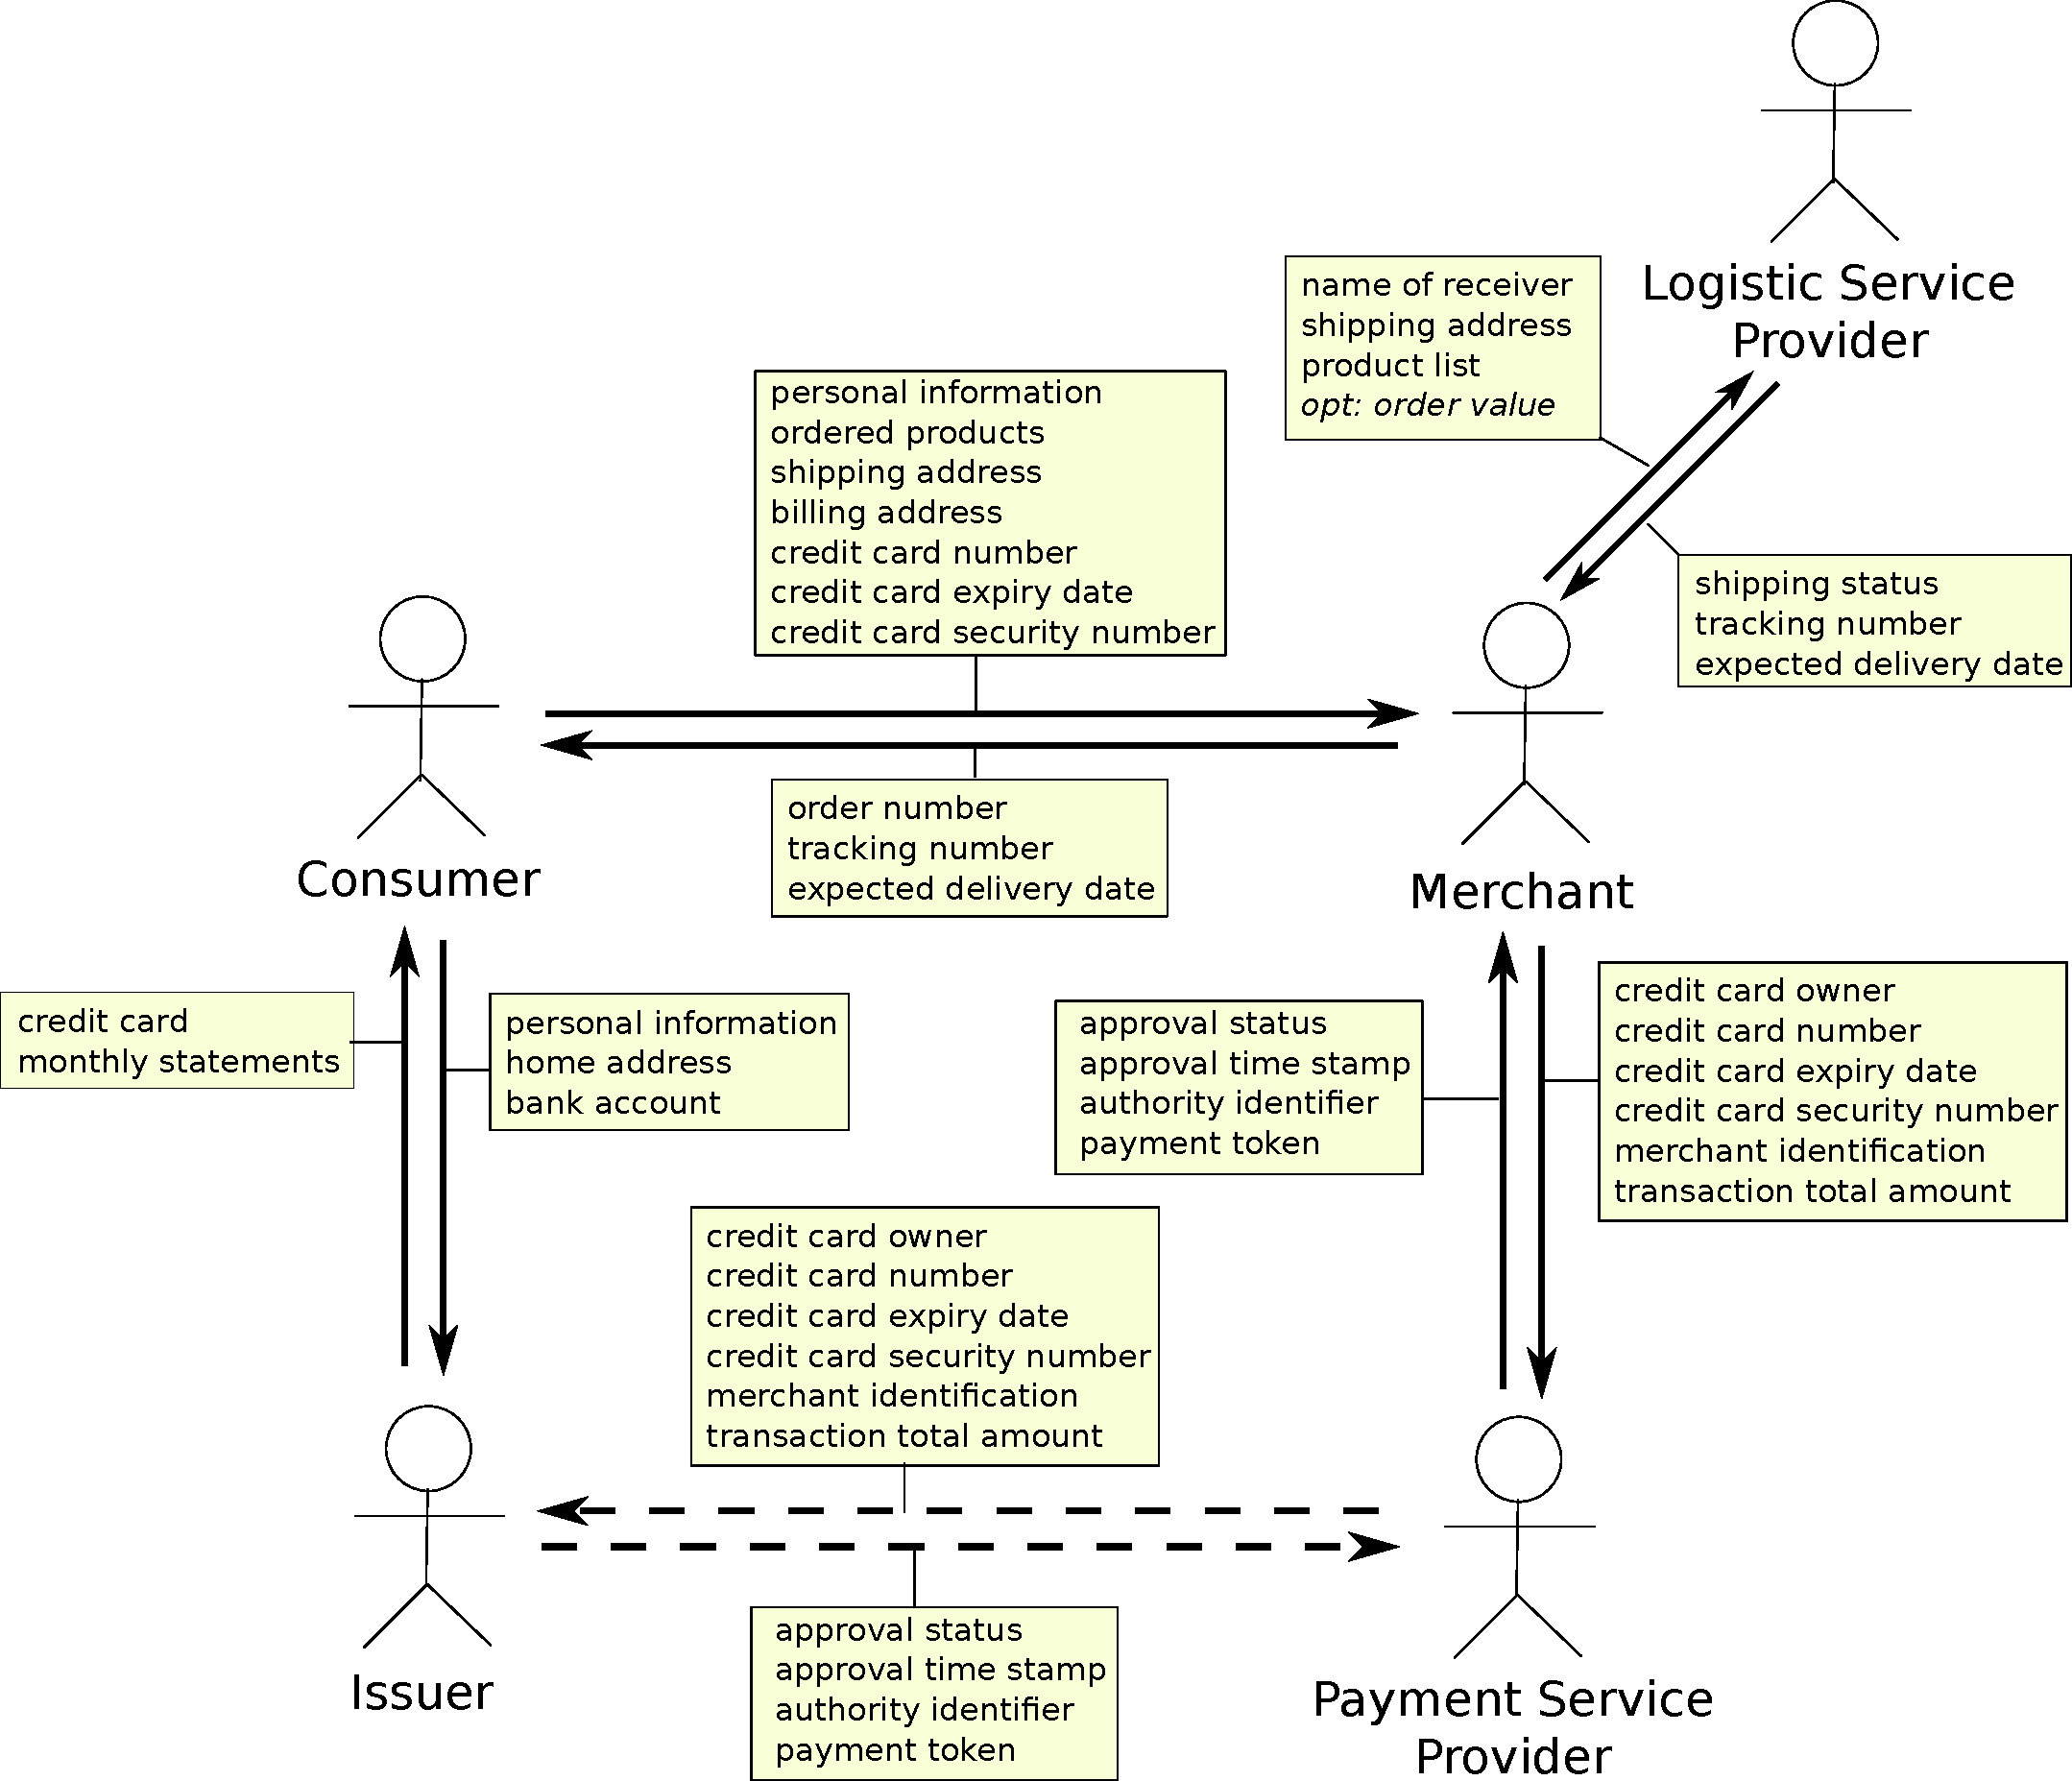
\includegraphics[width=0.8\columnwidth]{images/e-commerce-stakeholder.pdf}
	\caption{Stakeholder and Data Flow in \gls{E-commerce} scenario}
\label{fig:images_e_commerce_stakeholder}
\end{figure}
